\documentclass[a4paper, 12pt]{scrartcl}
\usepackage[utf8]{inputenc}
\usepackage[ngerman]{babel}
\usepackage{amsmath}
\usepackage{amssymb}
\usepackage{icomma}
\usepackage{graphicx}
\usepackage[pdftex]{hyperref}
\hypersetup{colorlinks=true, linkcolor=black, citecolor=black, filecolor=black, urlcolor=black, pdftitle={Datenblatt LAD-Spektrometer}}

\newcommand{\unit}[1]{\ensuremath{\,\mathrm{#1}}}
\setlength{\parindent}{0pt}
\setlength{\parskip}{\baselineskip}


\begin{document}
\begin{center}
\begin{Huge}
Datenblatt LAD-Spektrometer
\end{Huge}
\\[\baselineskip]
"`Light Absorbing Diodes"'
\end{center}


\section{Funktionsweise}
Das Spektrometer misst die relative Spektrale Leistungsdichte
\[
\frac
{\text{Leistung}}
{\text{Fläche}\cdot\text{Wellenlängenintervall}}
\]
im Bereich von $350\unit{nm}$ bis $750\unit{nm}$, also dem kompletten optischen Spektrum.
Es misst in 16 unabhängigen, ca. gleichverteilten überlappenden Kanälen und erreicht dabei eine spektrale Auflösung von ca. $40\unit{nm}$.
Verschiedene Lichtquellen sind somit ganz klar identifizierbar.



\section{Leuchtdioden}
Die verwendeten Leuchtdioden müssen einerseits das Spektrum gut abdecken und andererseits möglichst schmale Absorptionskurven besitzen.
Hierzu wurden in etwa 17 LEDs verschiedener Hersteller vermessen und selektiert.

Die folgenden LEDs sind im Spektrometer verbaut:

{\centering
\begin{tabular}{c|c|c|c|c|c}
\# & Hersteller & Typ & Vertrieb & Bestllnummer & $\lambda_\text{em} [\mathrm{nm}]$ \\
\hline
1 & & & Roithner & vl400 & 400\\
2 & & & Roithner & rlcv415 & 415\\
3 & Kingbright & KA-3529QB24ZS & Conrad & 180391 & 457\\
4 & Osram & Q65110A1987 & Reichelt & LVT67C & 505\\
5 & & & Roithner & epd470 & -\\
6 & Avago & HSMG-A100-J02J1 & Conrad & 180567 & 569\\
7 & Osram & Q65110A2399 & Reichelt & LPM675 & 560\\
8 & Osram & Q65110A4007 & Reichelt & LGT676 & 570\\
9 & Osram & Q65110A2156 & Reichelt & LYT676 & 587\\
10 & Avago & HSMU-A100-R00J1 & Conrad & 180575 & 592\\
11 & Kingbright & KA-3528IT & Reichelt & smd-led3528RT & 625\\
12 & & & Roithner & smc660 & 660\\
13 & & & Roithner & smc680 & 680\\
14 & & & Roithner & smc700 & 700\\
15 & & & Roithner & smt735 & 735\\
16 & & & Roithner & smc720 & 720\\
\end{tabular}}

Wir erhielten folgende Messwerte in Absorption.
Das Messwertsignal $I$ (offsetbereinigt) ist proportional zum eingebauten Messwiderstand $R$ und wurde im Sonnenspektrum gemessen.

{\centering
\begin{tabular}{c|c|c|c|c|c|c|c}
\# &
Bestllnummer &
$\lambda_\text{em} [\mathrm{nm}]$ &
$\lambda_\text{abs} [\mathrm{nm}]$ &
$\Delta\lambda_\text{abs} [\mathrm{nm}]$ &
$R [\mathrm{M\Omega}]$ &
$I [\text{ADUs}]$ &
$\Delta I$\\
\hline
1 & vl400 & 400 & 383 & 17\\
2 & rlcv415 & 415 & 397 & 14\\
3 & 180391 & 457 & 412 & 21\\
4 & LVT67C & 505 & 428 & 40\\
5 & epd470 & - & 482 & 43\\
6 & 180567 & 569 & 532 & 30\\
7 & LPM675 & 560 & 544 & 21\\
8 & LGT676 & 570 & 552 & 25\\
9 & LYT676 & 587 & 562 & 29\\
10 & 180575 & 592 & 578 & 23\\
11 & smd-led3528RT & 625 & 598 & 23\\
12 & smc660 & 660 & 627 & 29\\
13 & smc680 & 680 & 669 & 18\\
14 & smc700 & 700 & 680 & 22\\
15 & smt735 & 735 & 703 & 24\\
16 & smc720 & 720 & 704 & 17\\
\end{tabular}}

\begin{figure}[ht]
\centering
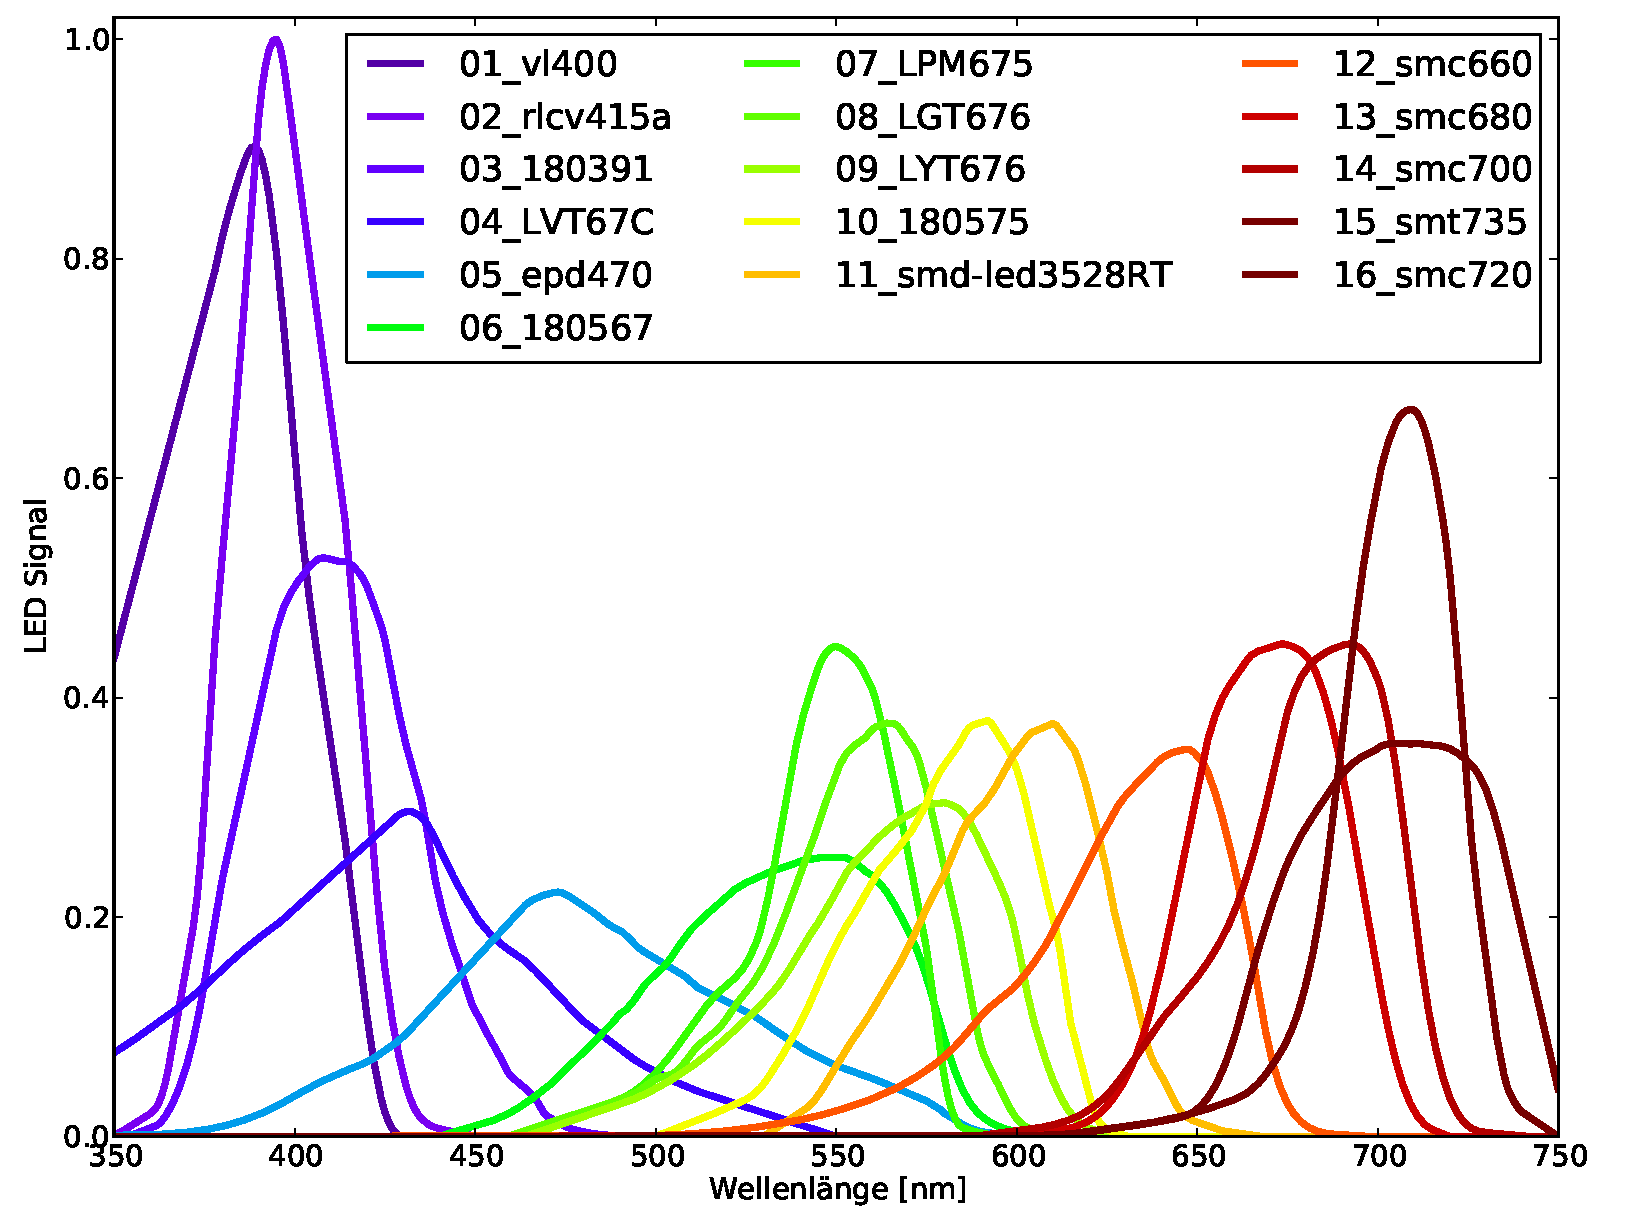
\includegraphics[width=\textwidth]{images/spektren.pdf}
\caption{Normierte Absorptionsspektren der eingebauten LEDs}
\end{figure}


\section{Kalibration}
Das Spektrometer ist mithilfe des Sonnenspektrums kalibriert. Es war keine bekanntere Lichtquelle vorhanden. Die Intensität des Sonnenspektrums wurde dabei von \url{http://rredc.nrel.gov/solar/spectra/am1.5/} genommen.


\section{Rekonstruktion}
Das mitgelieferte Auswertungsprogramm unterstützt drei Rekonstruktionsmodi.

\subsection{Backus Gilbert}
Dies ist ein generisches Rekonstruktionsverfahren, welches das komplette Spektrum möglichst original zu rekonstruieren versucht.
Backus-Gilbert ist dabei relativ unempfindlich gegenüber Schwankungen im Eingangssignal.
Dies lässt keine extrem scharfe Auflösung zu, ist aber notwendig aufgrund der vorhandenen Messwertschwankungen.
Das Verfahren ist beschrieben in "'Numerical Recipes"`, dritte Auflage, Kapitel 19.6.

\subsection{Schwarzkörper}
Ein Schwarzkörperspektrum mit den Parametern Temperatur und Amplitude wird auf die Messdaten gefittet und der Temperaturwert ausgegeben.

\subsection{Gauß}
Eine Gaußkurve mit den Parametern mittlere Wellenlänge, Breite und Amplitude wird auf die Messdaten gefittet und die mittlere Wellenlänge ausgegeben.

\end{document}
